\documentclass[zihao=false,fontset=windows]{ctexart}
% ctexart 不接受任意 pt 选项。正文改 {10pt}，方括号里是行距。
\usepackage{scrextend}
\changefontsizes[12pt]{10pt}

\usepackage[a4paper,left=2.35cm,right=2.35cm,top=1.7cm,bottom=1.9cm]{geometry}
\usepackage{xcolor}
\usepackage{graphicx}
\usepackage{amsmath,amssymb}
\usepackage{enumitem}
\usepackage{tabularx}
\usepackage{colortbl}
\usepackage{listings}
\usepackage{hyperref}
\usepackage[most]{tcolorbox}

\definecolor{feishuText}{RGB}{31,35,41}
\definecolor{feishuBlue}{RGB}{36,91,219}
\definecolor{feishuRed}{RGB}{216,57,49}
\definecolor{feishuGray}{RGB}{100,106,115}
\definecolor{feishuGray2}{RGB}{143,149,158}
\definecolor{feishuPinkBg}{RGB}{251,191,188}
\definecolor{quoteBar}{RGB}{51,112,255}
\definecolor{codebg}{RGB}{245,246,247}
\definecolor{codeborder}{RGB}{222,224,227}
\definecolor{inlinebg}{RGB}{242,243,245}
\definecolor{callRed}{RGB}{253,226,226}
\definecolor{callOrange}{RGB}{255,245,235}
\definecolor{callYellow}{RGB}{254,255,240}
\definecolor{callGreen}{RGB}{240,251,239}
\definecolor{callBlue}{RGB}{240,244,255}
\definecolor{callRedSoft}{RGB}{254,241,241}
\definecolor{callSun}{RGB}{255,255,204}
\definecolor{tableHead}{RGB}{242,243,245}
\definecolor{tableRule}{RGB}{222,224,227}
\definecolor{codeText}{RGB}{31,35,41}
\definecolor{codeKeyword}{RGB}{0,0,255}
\definecolor{codeComment}{RGB}{0,128,0}
\definecolor{codeString}{RGB}{163,21,21}

\setmainfont{Times New Roman}
\setCJKmainfont{Microsoft YaHei}[AutoFakeBold=2.2]
\setCJKsansfont{Microsoft YaHei}[AutoFakeBold=2.2]
\setCJKmonofont{Microsoft YaHei}[AutoFakeBold=2.2]
\setmonofont{Consolas}
\newfontfamily\emojifont{Segoe UI Emoji}

\hypersetup{
  colorlinks=true,
  urlcolor=feishuBlue,
  linkcolor=feishuBlue,
  unicode=true,
  pdftitle={SigLIP}
}

\setlength{\parindent}{0pt}
\setlength{\parskip}{0.42em}
\setlength{\fboxsep}{1.5pt}
\setlength{\emergencystretch}{3em}
\linespread{1.28}
\color{feishuText}
\arrayrulecolor{tableRule}
\urlstyle{same}

\setlist[enumerate]{label=\textcolor{feishuBlue}{\arabic*.}, leftmargin=1.7em, itemsep=0.22em, topsep=0.28em, parsep=0.08em, partopsep=0pt}
\setlist[itemize,1]{label=\textcolor{feishuBlue}{\textbullet}, leftmargin=1.35em, itemsep=0.18em, topsep=0.25em, parsep=0.06em, partopsep=0pt}
\setlist[itemize,2]{label=\textcolor{feishuBlue}{◦}, leftmargin=1.45em, itemsep=0.12em, topsep=0.15em}
\setlist[itemize,3]{label=\textcolor{feishuBlue}{\rule[0.18em]{0.38em}{0.38em}}, leftmargin=1.55em, itemsep=0.1em, topsep=0.12em}

\newcommand{\feiEmoji}[1]{{\emojifont #1}}
\newcommand{\incode}[1]{\colorbox{inlinebg}{\ttfamily\small #1}}
\newcommand{\bigmath}[1]{%
  \begin{center}\large$\displaystyle #1$\end{center}%
}

\lstset{
  language=Python,
  basicstyle=\ttfamily\footnotesize\color{codeText},
  keywordstyle=\color{codeKeyword},
  commentstyle=\color{codeComment},
  stringstyle=\color{codeString},
  showstringspaces=false,
  breaklines=true,
  columns=fullflexible,
  keepspaces=true,
  tabsize=4,
  upquote=true,
  aboveskip=2pt,
  belowskip=0pt,
  xleftmargin=0pt,
  frame=none
}

\tcbset{
  feishubase/.style 2 args={
    enhanced,
    boxrule=0pt,
    arc=8pt,
    left=10pt,
    right=10pt,
    top=7pt,
    bottom=7pt,
    before skip=6pt,
    after skip=6pt,
    colback=#1,
    colframe=#1,
    before upper={\feiEmoji{#2}\hspace{0.45em}\ignorespaces}
  }
}
\newtcolorbox{feishubox}[2]{feishubase={#1}{#2}, breakable}
\newtcolorbox{feishuboxnb}[2]{feishubase={#1}{#2}}

\newtcolorbox{feishuquote}{
  enhanced,
  breakable,
  boxrule=0pt,
  leftrule=3pt,
  arc=0pt,
  colframe=quoteBar,
  colback=white,
  left=8pt,
  right=2pt,
  top=2pt,
  bottom=2pt,
  before skip=4pt,
  after skip=4pt,
  before upper=\color{feishuGray}
}

\newtcolorbox{feishucode}{
  enhanced,
  breakable,
  colback=codebg,
  colframe=codeborder,
  boxrule=0.6pt,
  arc=6pt,
  left=6pt,
  right=6pt,
  top=5pt,
  bottom=4pt,
  before skip=6pt,
  after skip=6pt
}


\usepackage{needspace}
% 来源：https://scnajei2ds6y.feishu.cn/wiki/IAqAwbiLVi0gEOkC87Qc0hAVnPe
% 公式依据网页渲染及公式原图人工转写并视觉核对。

\begin{document}

{\zihao{1}\bfseries SigLIP\par}

\begin{feishubox}{callOrange}{📒}论文：《Sigmoid Loss for Language Image Pre-Training》\par 论文链接：\href{https://arxiv.org/pdf/2303.15343}{https://arxiv.org/pdf/2303.15343}\par GitHub：\href{https://link.zhihu.com/?target=https\%3A//github/}{https://github}\href{https://link.zhihu.com/?target=https\%3A//github/}{. com/google-research/big\_vision}\end{feishubox}

\par\needspace{5\baselineskip}\vspace{1em}\noindent{\zihao{-2}\bfseries \textcolor{feishuBlue}{1.} 背景}\par\vspace{0.28em}

\href{https://scnajei2ds6y.feishu.cn/wiki/FKvTwjSHxiVHBokxd5ncXxuanch}{CLIP(2021, OpenAI)} 和 \href{https://proceedings.mlr.press/v139/jia21b.html}{ALIGN} 使用大量若监督文本对实现对比学习，标准的做法是使用图像-文本对比目标：拉近嵌入空间中的匹配（正）图像-文本表示，同时远离嵌入空间中无关（负）图像-文本表示。\par

即，给定一个包含图像-文本对的小批量$B=\{(I_1,T_1),(I_2,T_2),\ldots\}$，对比学习的目标是鼓励匹配对 $(I_i,T_i)$ 的嵌入相互对齐，同时将不匹配对 $(I_i,T_{j\neq i})$ 的嵌入分开。\par

\begin{feishubox}{callOrange}{🤔}\textcolor{feishuRed}{\textbf{以上有一个noisy and imperfect的假设：对于所有图像 }}{\boldmath $i$}\textcolor{feishuRed}{\textbf{ ，与另一图像 }}{\boldmath $j$}\textcolor{feishuRed}{\textbf{ 相关联的文本与 }}{\boldmath $i$}\textcolor{feishuRed}{\textbf{ 无关，反之亦然。}}\end{feishubox}

但是基于softmax的对比学习存在两个问题：\par

\begin{itemize}

\item \href{https://scnajei2ds6y.feishu.cn/wiki/FKvTwjSHxiVHBokxd5ncXxuanch}{CLIP(2021, OpenAI)} 的 loss 是 batch-level softmax-based 的，softmax不对称，导致需要分别对图像和文本 normalize the pairwise similarity scores，即：

\bigmath{-\frac{1}{2|B|}\sum_{i=1}^{|B|}(\overbrace{\log\frac{e^{t \mathbf{x}_i\cdot \mathbf{y}_i}}{\sum_{j=1}^{|B|}e^{t \mathbf{x}_i\cdot \mathbf{y}_j}}}^{\text{image}\to\text{text softmax}}+\overbrace{\log\frac{e^{t \mathbf{x}_i\cdot \mathbf{y}_i}}{\sum_{j=1}^{|B|}e^{t \mathbf{x}_j\cdot \mathbf{y}_i}}}^{\text{text}\to\text{image softmax}})}

其中$\mathbf{x}_i=\frac{f(I_i)}{\|f(I_i)\|_2}$和$\mathbf{y}_i=\frac{g(T_i)}{\|g(T_i)\|_2}$。并且 $\text{image model 表示为 }f(\cdot)\text{ 并且 text model 表示为 }g(\cdot)$。\par

\item 为了防止softmax计算溢出，需要对每一个值减去当前batch对最大值，因此需要一次预先的遍历。

\end{itemize}

\par\needspace{5\baselineskip}\vspace{1em}\noindent{\zihao{-2}\bfseries \textcolor{feishuBlue}{2.} SigLIP}\par\vspace{0.28em}

\par\needspace{5\baselineskip}\vspace{1em}\noindent{\zihao{3}\bfseries \textcolor{feishuBlue}{2.1} 计算方法}\par\vspace{0.28em}

SigLIP是一种更简单的替代方案，利用Sigmoid代替基于softmax的对比损失，这种方案\textbf{无需计算全局归一化因子。}\par

基于Sigmoid的损失独立地处理每一个图像-文本对，有效地将学习问题转化为在所有对组合的数据集上的标准二分类问题，其中匹配对 $(I_i,T_i)$ 标记为正例，而所有其他对 $(I_i,T_{j\neq i})$ 标记为负例。其定义如下：\par

\bigmath{-\frac{1}{|B|}\sum_{i=1}^{|B|}\sum_{j=1}^{|B|}\underbrace{\log\frac{1}{1+e^{z_{ij}(-t \mathbf{x}_i\cdot \mathbf{y}_j+b)}}}_{\mathcal L_{ij}}}

其中 $z_{ij}$ 是给定图像和文本输入的标签，如果它们是匹配的则等于1，否则等于-1。\par

在初始化阶段，来自众多负例的严重不平衡主导了损失，导致初始优化步骤试图修正这种偏差。为了缓解这一点，SigLIP 引入了一个额外的可学习偏置项 $b$ ，类似于温度 $t$ 。我们将 $t'$ 和 $b$ 分别初始化为 $\log 10$和 $-10$ 。这确保了训练大致从先验值附近开始，而无需进行大幅度的过度修正。\par

\needspace{19\baselineskip}算法伪代码：\par

\begin{center}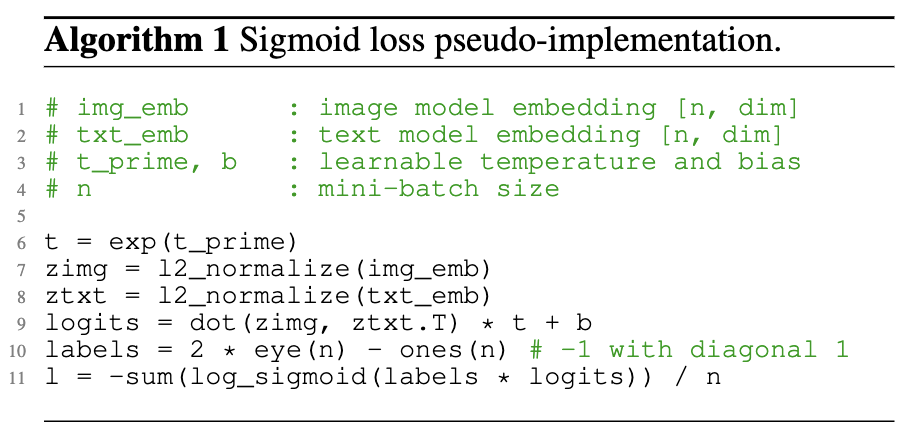
\includegraphics[width=0.78\linewidth]{images/SigLIP/fig-01.png}\end{center}

\par\needspace{5\baselineskip}\vspace{1em}\noindent{\zihao{3}\bfseries \textcolor{feishuBlue}{2.2} 高效分块(chunked)计算}\par\vspace{0.28em}

对比训练通常使用Data Parallel。当数据分布在$D$个设备上时计算损失，需要收集所有嵌入来计算每一个pair之间的cosine相似度，这涉及到昂贵的all-gathers操作，更重要的是，需要实例化一个内存密集型的 $|B|\times|B|$ 两两相似度矩阵。\par

\textbf{Sigmoid损失特别适合于一种内存高效}，快速且数值稳定的实现方式，这种方式改善了上述两个问题。将每个设备上的批量大小表示为 $b=\frac{|B|}{D}$ ，损失可以重新表述为：\par

\bigmath{-\frac{1}{|\mathcal B|}
\underbrace{\sum_{d_i=1}^{D}}_{\text{A: }\forall\text{ device }d_i}
\overbrace{\sum_{d_j=1}^{D}}^{\substack{\text{B: swap negs}\\\text{across devices}}}
\overbrace{\underbrace{\sum_{i=bd_i}^{b(d_i+1)}}_{\substack{\text{all local}\\\text{positives}}}
\underbrace{\sum_{j=bd_j}^{b(d_j+1)}}_{\substack{\text{negs from}\\\text{next device}}}}^{\substack{\text{C: per device}\\\text{loss}}}\mathcal L_{ij}}

简单来说，首先计算对应于正例对以及$b-1$个负例对的损失部分，然后，跨设备置换embedding，以便每个设备从其相邻设备获取负例（求和B）。然后根据这个分块（求和C）计算损失。这是在每个设备上独立完成的，因此每个设备根据其本地批量$b$计算损失。然后，可以在所有设备上简单地将损失相加（求和A）。\par

这个过程的示意图如图，这个过程和\href{https://zhuanlan.zhihu.com/p/504957661}{Ring All-reduce}是类似的：\par

\begin{center}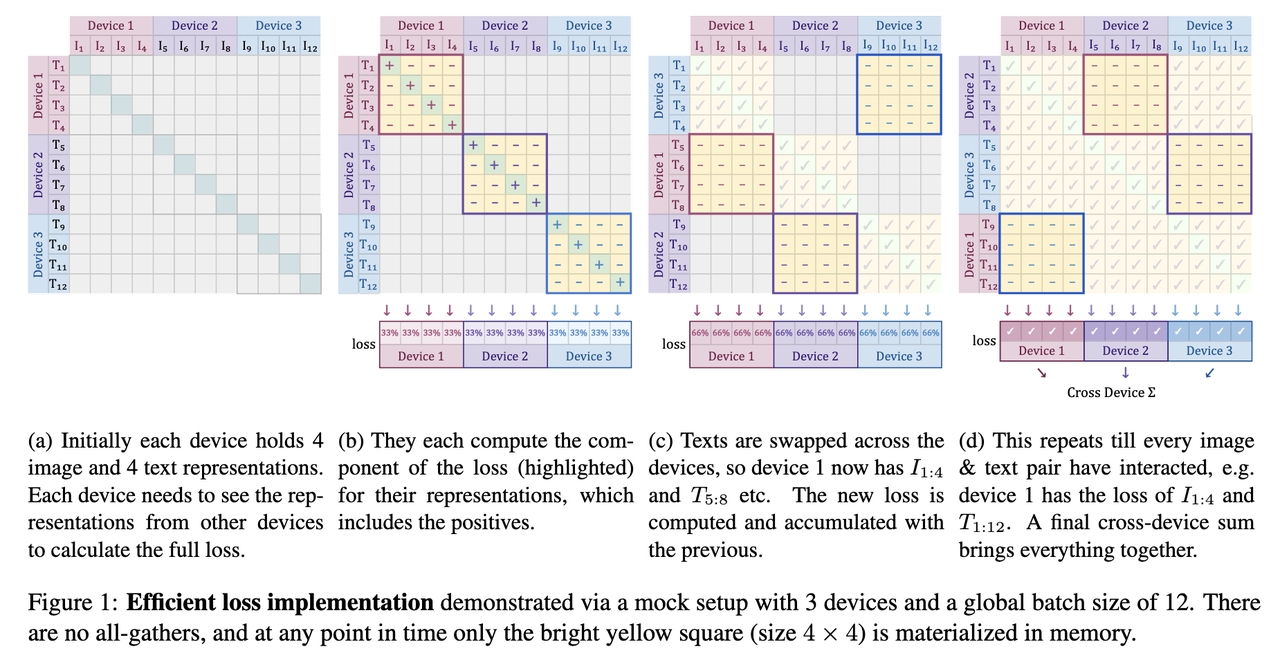
\includegraphics[width=0.98\linewidth]{images/SigLIP/fig-02.png}\end{center}

\textbf{在任何给定时刻的内存成本从 }{\boldmath $|B|^2$}\textbf{ 降低到了 }{\boldmath $b^2$}\textbf{，使SigLIP能够在相对较少的设备上实现超过一百万的批量大小进行训练。}\par

\par\needspace{5\baselineskip}\vspace{1em}\noindent{\zihao{-2}\bfseries \textcolor{feishuBlue}{3.} 实验}\par\vspace{0.28em}

与其他公开发布的模型的比较，SigLIP模型在零样本分类和检索任务上均以显著优势超越所有先前的模型，例如OpenCLIP和CLIP。与同期的EVA-CLIP和CLIPA-v2相比，SigLIP-L在低分辨率和高分辨率情况下全面表现出更佳性能\par

\begin{center}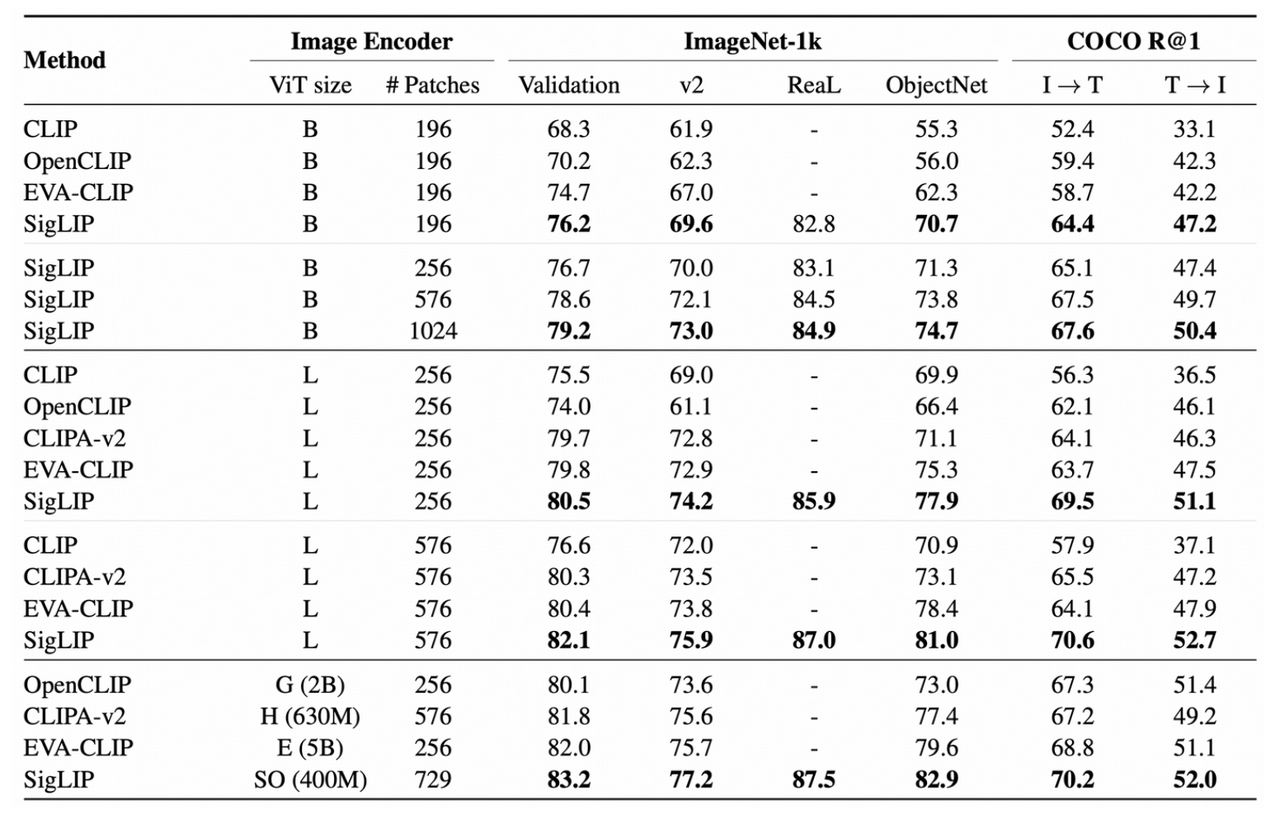
\includegraphics[width=0.86\linewidth]{images/SigLIP/fig-03.png}\end{center}

\end{document}
